\label{taxi-reservation}
\subsubsection{Purpose}

Any subscribed passenger shall be able to reserve a taxi for a ride at a predefined time. The passenger has to specify in advance the origin and the destination of the ride, along with the starting date and time and the number of passengers.

The passenger can also enable the sharing mode for the ride.
In that case, also the requirement in~\autoref{ride-sharing} apply.

\begin{figure}
	\begin{center}
	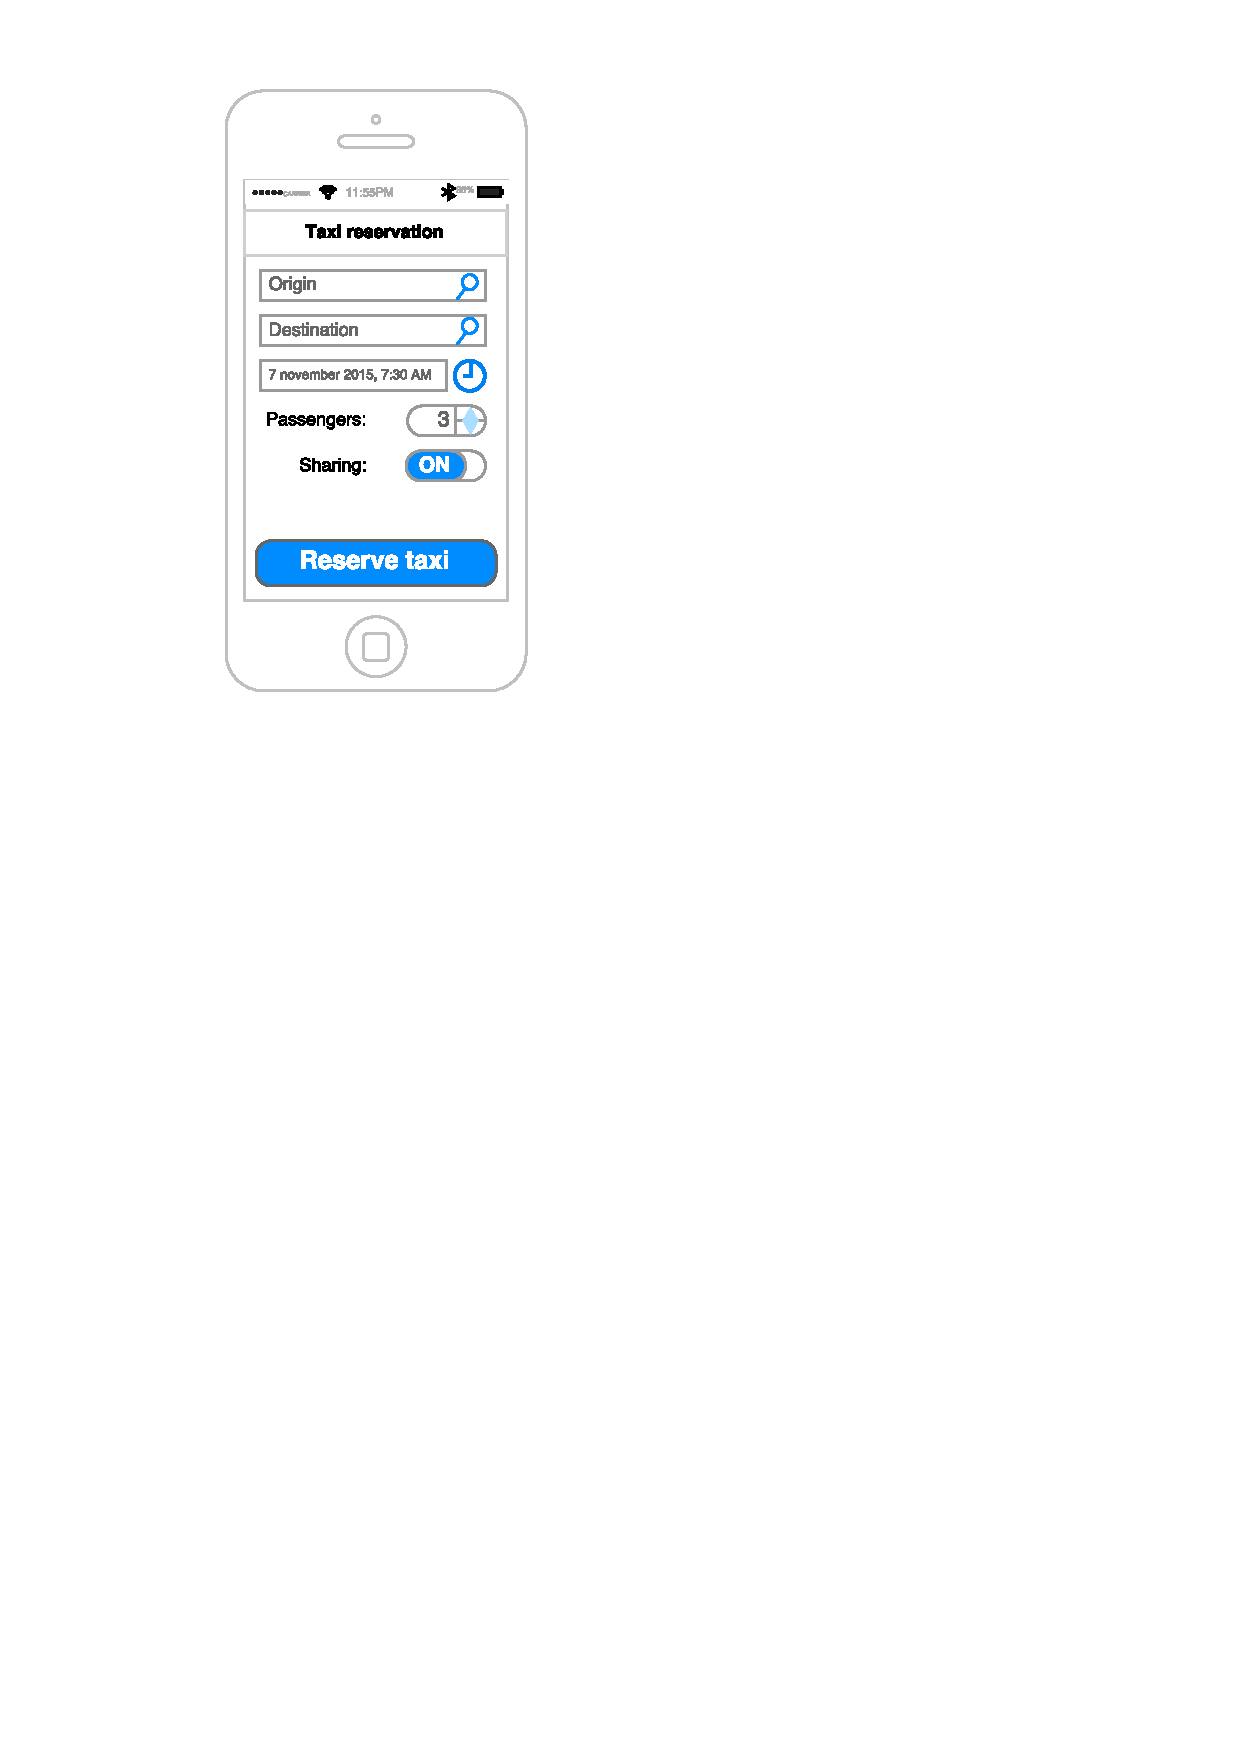
\includegraphics[width=0.5\textwidth]{mockup/TaxiReservation.pdf}
	\caption{Concept of the taxi reservation screen on the mobile application.}
	\label{fig:mockup-reservation}
	\end{center}
\end{figure}

\subsubsection{Scenario 1}
John McClane will need a taxi to get to the airport tomorrow morning. He opens the web application of myTaxiService and decides to book a taxi for 6:00 AM for a ride from his home to the airport, for 1 person. He confirms the request.

The morning after, at 5:40 AM, the first taxi driver in the queue gets McClane's request and accepts it. He comes to pick up McClane and brings him to the airport.

\subsubsection{Scenario 2}
Cordell Walker needs to get to the Texas Rangers police station tomorrow morning.
His pick-up truck needs to be repaired, so he reserves a taxi for 7:30 AM. He enables the sharing option.
No one wants to go to the Texas Rangers in the same zone at the same hour for now, so Walker becomes the owner of the ride.

Trivette, who doesn't have a car, also needs to go to the Texas Rangers station, and tries to reserve a taxi with the sharing option.
The systems informs him that a shared ride with his colleague Walker is available. He accepts.

In the morning, the taxi driver gets called at 7:10 AM and goes to Walker's place.
Trivette reaches the starting point, where the taxi driver picks up Walker and Trivette and leaves them by the Texas Rangers.

\subsubsection{Use case}
The use case for a taxi reservation is shown in~\autoref{usecase-reservation}.

\begin{table}
\begin{center}
\begin{tabular}{| l | p{0.6\textwidth} |}
\hline
Actor & Passenger \\
\hline
Goal & Goal~\ref{g-reserve}
\\
\hline
Input condition & Passenger is already logged in and chooses to reserve a taxi.  \\
\hline
Event Flow & \begin{enumerate}
	\item The passenger chooses to reserve a taxi using his client.
	\item The passenger chooses the origin and destination addresses, the number of travelers, and the time of pick-up.
	\item The passenger confirms the reservation.
	\item 10 minutes prior to the ride time, the request gets forwarded to the first taxi in the queue of the same taxi zone of the user.
	\item The taxi driver can either accept or deny the request; if he denies it, the request is forwarded to the next taxi driver in the queue, and so on.
	\item Finally the request gets accepted by a taxi driver.
	\item The passenger gets notified that a taxi driver accepted his request and is given the ETA of the incoming taxi.
	\item When the taxi driver meets the passenger, he/she signals that the passenger is on board.
\end{enumerate}
\\
\hline
Output condition & The driver confirms that the passenger is aboard. \\
\hline
Exception & No taxi is available in the passenger's zone. \\
\hline
\end{tabular}
\end{center}
\caption{Use case for taxi reservation.}
\label{usecase-reservation}
\end{table}

\subsubsection{Response sequence}
The response sequence for a simple taxi reservation is illustrated in~\autoref{fig:sequence-taxireservation}.
The statechart of a taxi reservation with ride sharing is shown in~\autoref{fig:sequence-reservation-sharing}
\begin{figure}
	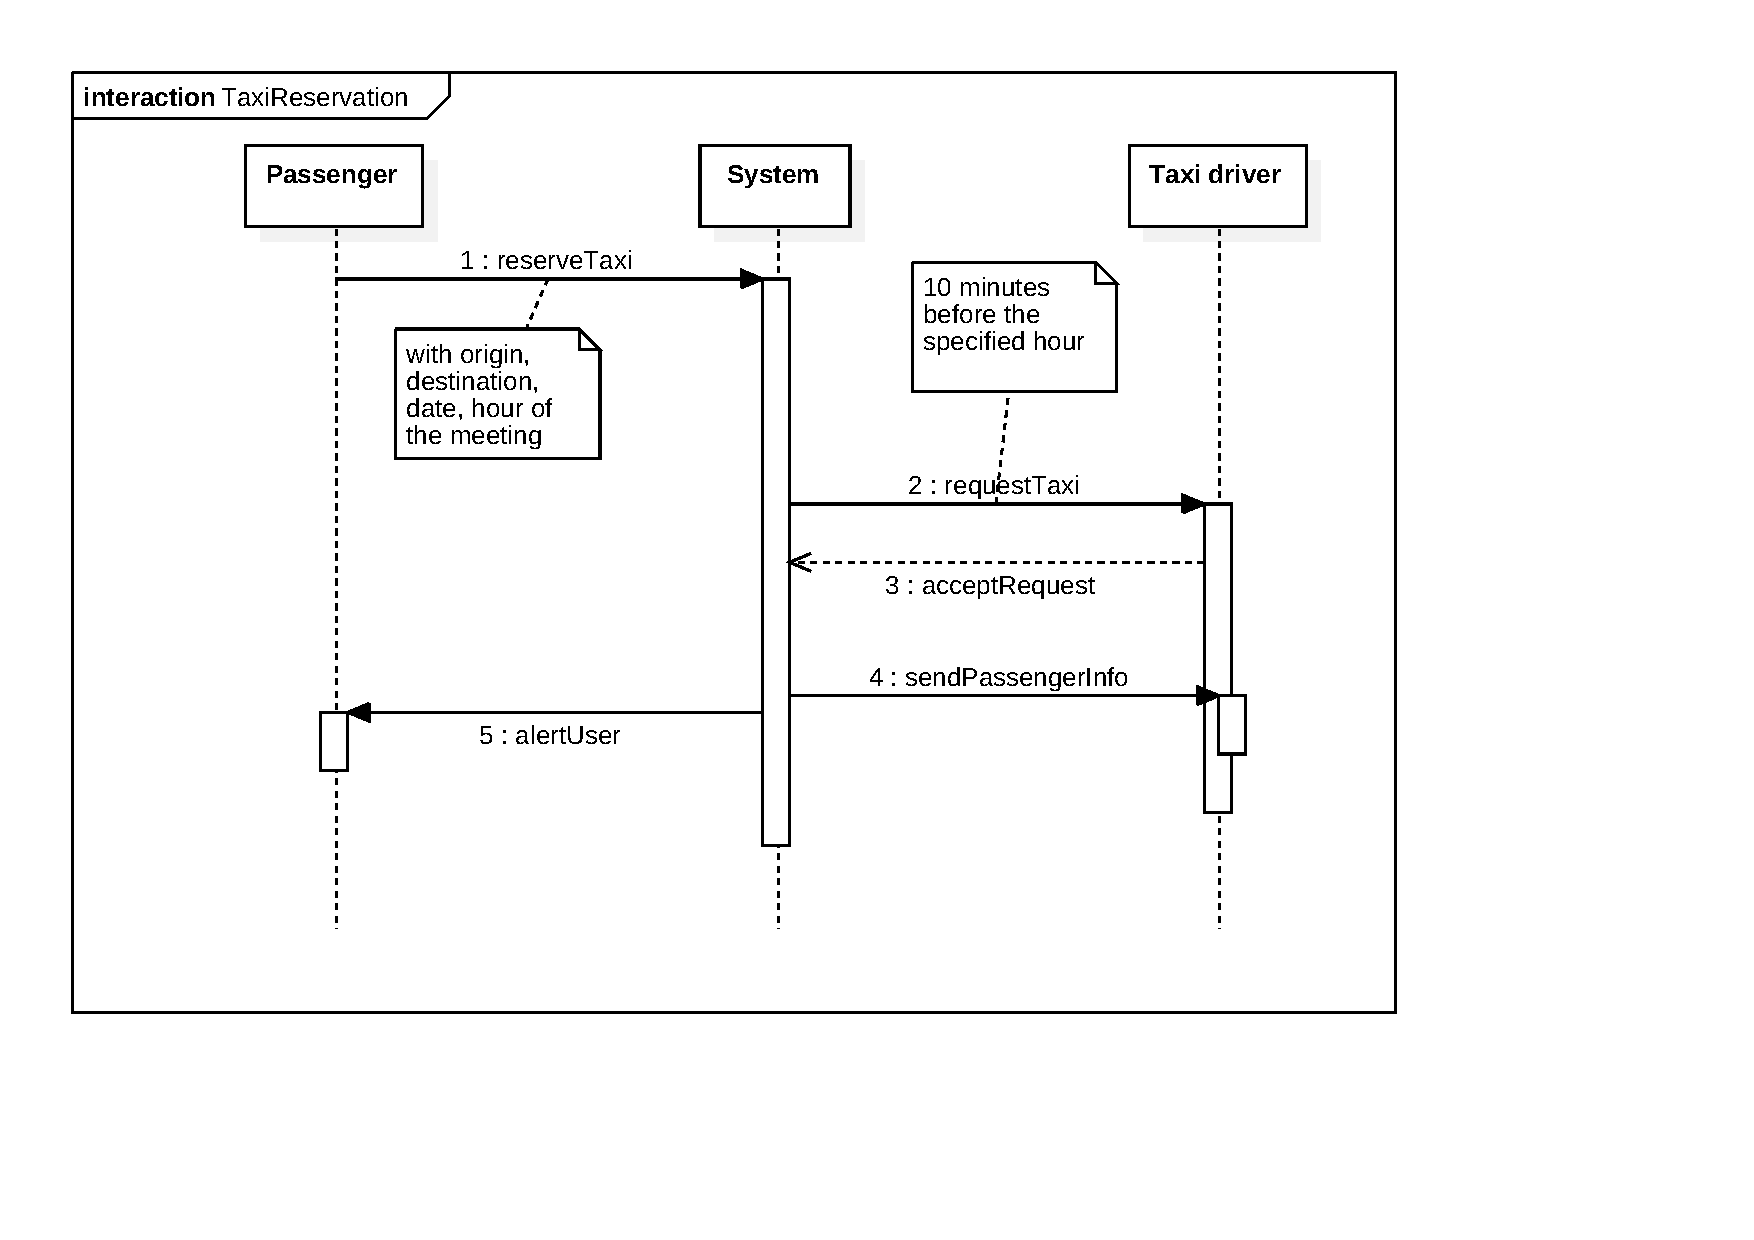
\includegraphics[width=\textwidth]{diagrams/sequence_taxireservation.pdf}
	\caption{Sequence diagram of a successful taxi reservation.}
	\label{fig:sequence-taxireservation}
\end{figure}

\begin{figure}
	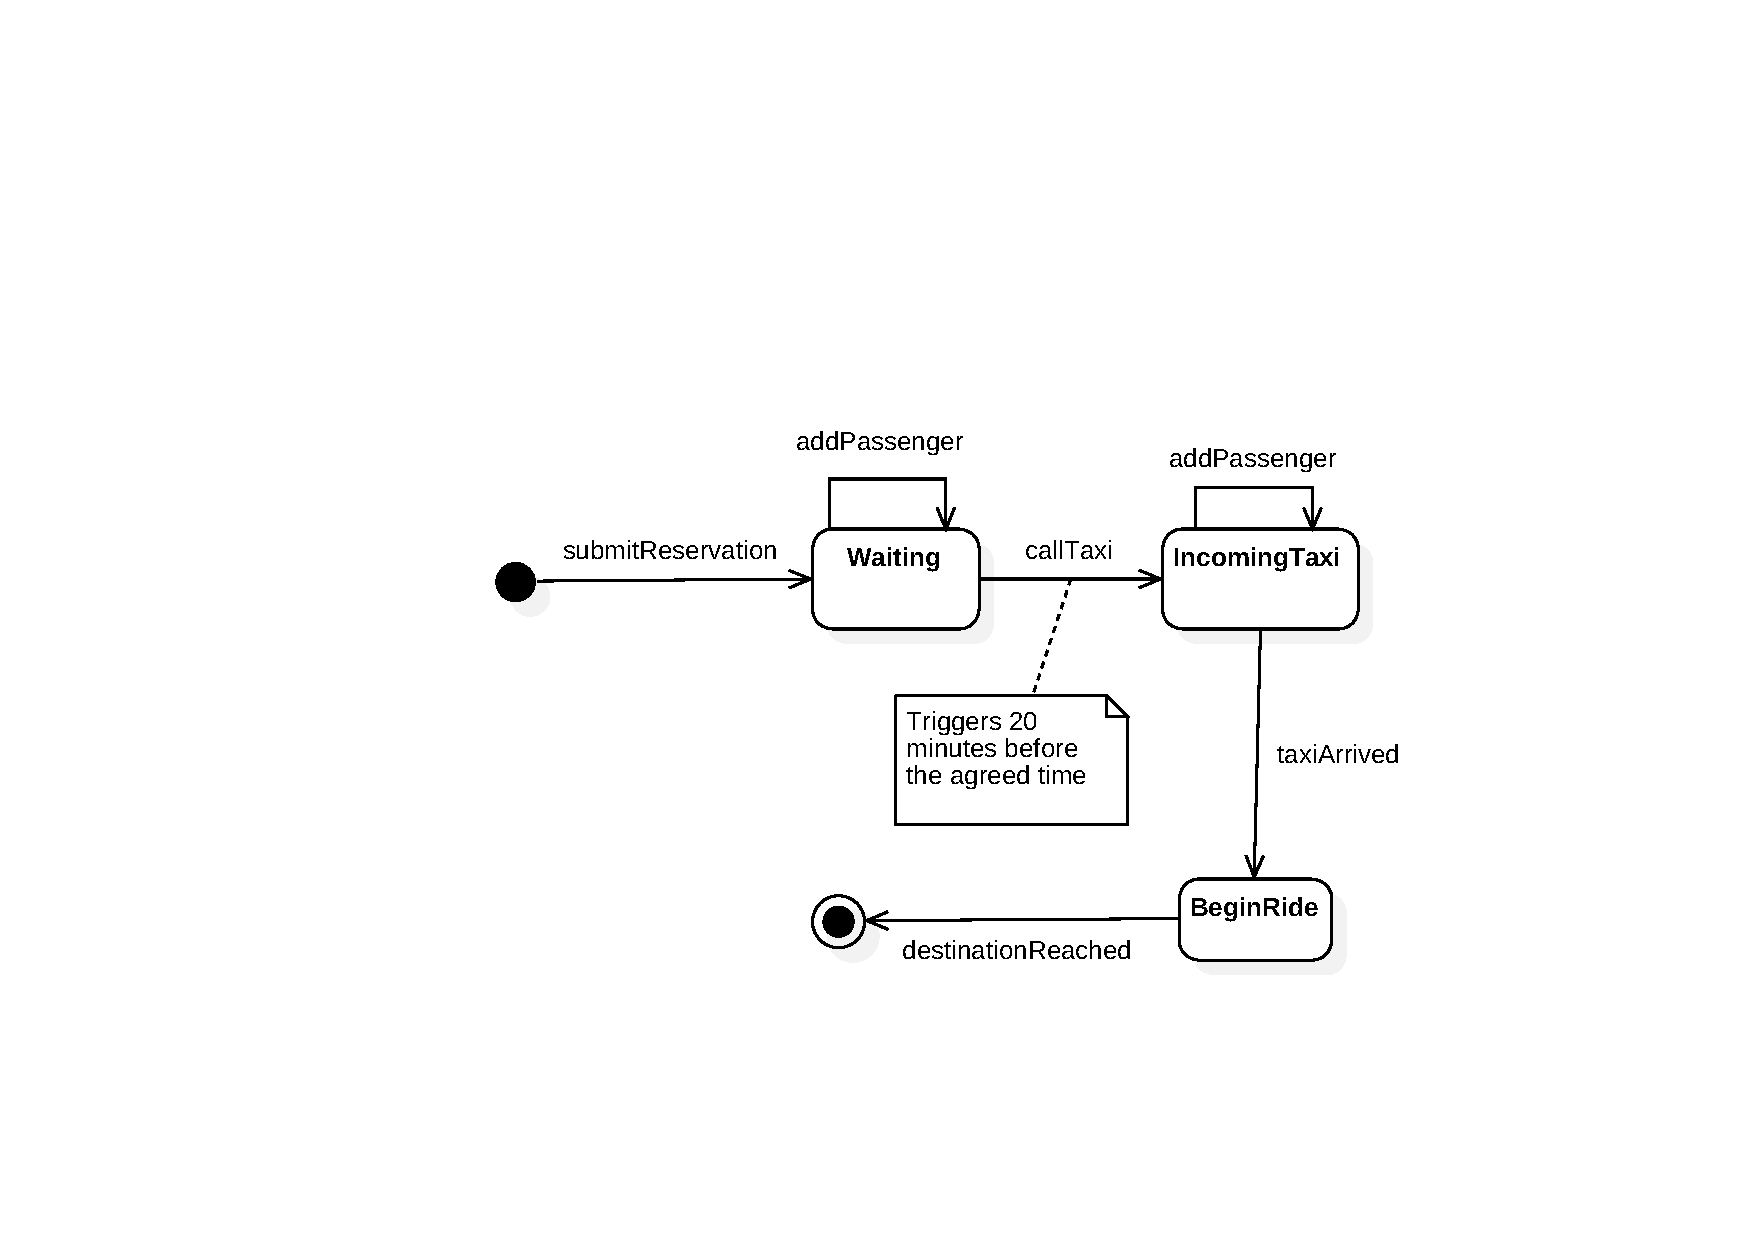
\includegraphics[width=\textwidth]{diagrams/statechart_reservation_shared.pdf}
	\caption{Statechart of a taxi reservation with ride sharing.}
	\label{fig:sequence-reservation-sharing}
\end{figure}

\subsubsection{Associated functional requirements}
\begin{enumerate}
	\item The system presents the passenger with the option to reserve a taxi.
	\item The system asks the passenger the origin and the destination of the ride.
	\item The system asks the passenger the total number of travelers.
	\item Origin and destination must be valid addresses.
	\item If GPS info is present and accurate within 50 m, the passenger can specify ``current position'' as the destination of the ride.
	\item The system asks the passenger the date and time of the ride.
	\item The system lets the passenger enter only valid dates and times.
	\item The system lets the passenger reserve a taxi from 48 hours to 2 hours before the actual ride time.
	\item 20 minutes before the specified arriving time, the system allocates a taxi for the passenger by putting a request in the queue as described in subsection~\ref{standard-call}.
	\item If no taxi is available at that time, the system keeps retrying until a taxi is available.
	\item After the request is accepted, the passenger gets notified with the ETA of the incoming taxi along with its position.
	\item The system must prevent the passenger from reserving more than one taxi per hour.
	\item A reserved ride can be shared.
	\item If the ride is shared, other passengers (with their travelers) can join the ride since it is submitted to the system.
	\item If the ride if shared, requirements in~\autoref{ride-sharing} apply.
\end{enumerate}
